\section{Estudo de Caso}\label{sec:estudo-de-caso}

A aplicação abordada nesse trabalho têm demandas semelhantes, porém não idênticas, em relação a outros sistema de localização. Antes de escolher uma tecnologia de posicionamento versátil apropriada, as propriedades comuns devem ser analisadas. Na etapa subsequente, o desempenho exigido de acordo com a aplicação individual deve ser analisado. São características do ambiente a ser executada a aplicação:

\begin{itemize}
    \item O ambiente onde a localização é realizada é conhecido de antemão e, portanto, pode estar preparado para apoiar ativamente o posicionamento. Ou seja, unidades de referência fixas podem ser implantadas neste ambiente, a partir da interação da qual a localização de um alvo móvel pode ser derivada; 
    \item Um modelo de localização geométrico 2D ou 3D pode ser aplicado para descrever informações de localização. Esse modelo pode ser um sistema de coordenadas cartesiano ou polar local, fornecendo coordenadas x, y e z, ou latitude, longitude e altitude, respectivamente;
    \item A escala do sistema não excede algumas dezenas de metros. Os sistemas de localização limitados a uma área relativamente pequena são frequentemente referidos como sistemas de posicionamento local (LPS), a fim de distingui-los explicitamente de implementações em larga escala como sistemas de posicionamento de rede celular 2G/3G ou sistemas de navegação global por satélite (GNSS). Os sistemas internos caem na categoria LPS por natureza;
    \item o posicionamento pode ser realizado usando métodos de localização relativa ou absoluta, ou ambos.
\end{itemize} 

\subsection{Objetivo}
Realizar uma análise quantitativa de forma a avaliar e validar a eficiência em relação aos parâmetros de desempenho. Esses dados foram obtidos fazendo um comparativo entre o cenário real e os dados indicados pela solução. Para tal foi utilizada a técnica de estudo experimental \textit{In Virtuo}. Essas medidas estão listadas no seguinte: 

\begin{itemize}
    \item Um dos principais parâmetros de desempenho de um sistema de localização é a sua exatidão. Este termo indica até que ponto a localização estimada se desvia da localização verdadeira. A exatidão é muitas vezes confundida com precisão. A precisão é uma medida da reprodutibilidade de uma medição. Portanto, quando uma declaração é feita sobre a resolução de um sistema de localização, a exatidão é geralmente complementada por precisão (por exemplo, precisão de 20 cm em mais de 90\% do tempo).
    \item O custo é um problema crítico, particularmente em aplicações onde várias unidades precisam ser equipadas com tecnologia de localização. Por conseguinte, é razoável utilizar componentes padrão de baixo custo sempre que possível. Além dos objetivos móveis, os custos de infraestrutura, implantação e manutenção devem ser considerados.
    \item A tecnologia utilizada deve ser compatível com seres humanos que trabalham ou vivem dentro do alcance do sistema de localização. 
\end{itemize} 

\subsection{Método}
foi realizado um estudo de caso, baseado em pesquisa experimental pois há um alto nível de controle da situação e do ambiente, permitindo isolar todas as estruturas de qualquer interferência do meio exterior, gerando maior confiabilidade nos resultados.

A avaliação ocorreu seguindo o fluxo:

\begin{enumerate}
\item Adicionar o \textit{Kinect} em um ponto estratégico da sala;
\item Iniciar o sistema produto da solução;
\item Avaliar entrada e saída de um grupo distinto de pessoas em momentos distintos e ao mesmo tempo;
\item Comparar os dados obtidos pela solução com o ocorrido nas cenas durante a avaliação;
\item Calcular a eficiência de acordo com os dados obtidos dessa comparação;
\item Comparar os resultados com outras tecnologias de detecção \textit{indoor}.
\end{enumerate}

\subsection{Resultados}
Os resultados obtidos da análise em questão podem ser vistos na Figura \ref{fig:results}. À esquerda, no console, podemos identificar os dados impressos, posicionamento $X$, $Y$,$Z$ e a distancia para o \textit{Kinect}. À direita, a exibição do \textit{MainWindow.xaml}, exibindo o mapa de profundidade e uma máscaras de triângulos, identificando a região da face do indivíduo. A Tabela \ref{table:comparativotecnologias} no Apêndice \ref{sec:apendiceB} exibe um comparativo entre as tecnologias atuais de detecção de localização e a solução desenvolvida.

\begin{figure*}[ht]
\centering
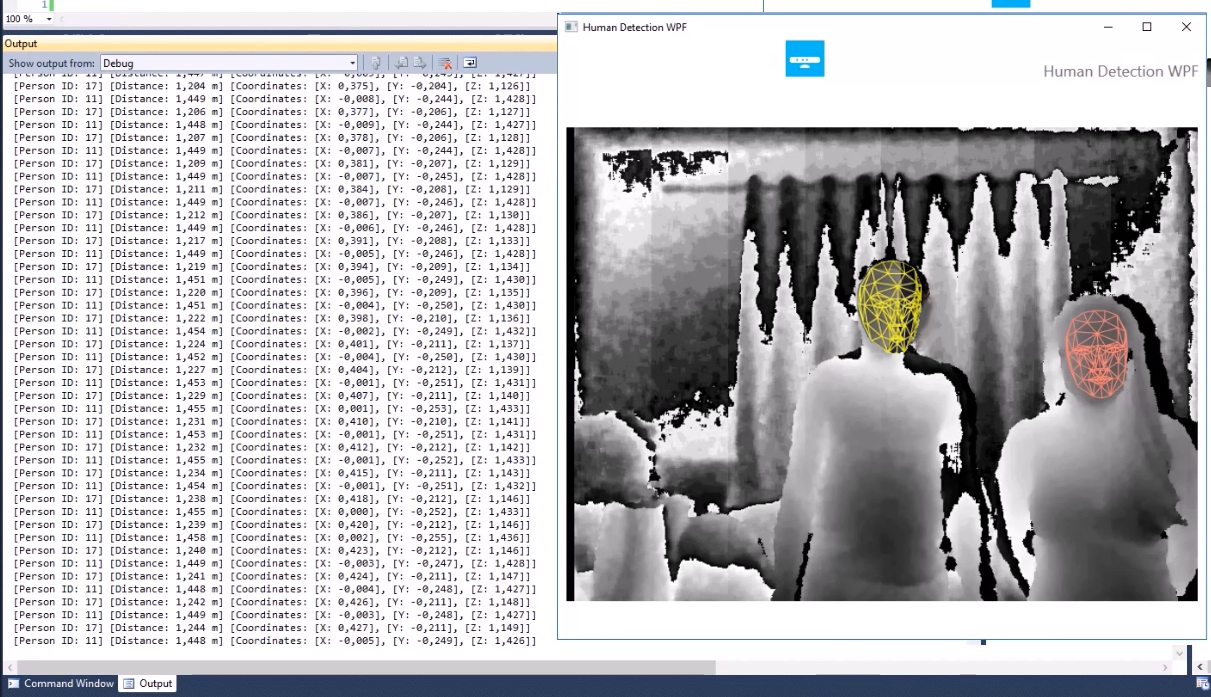
\includegraphics[width=1.0\textwidth]{images/detection01.png}
\caption{Aplicação em execução. Detecção e resultados: à esquerda são exibidos o posicionamento e distância e à direita o mapa de profundidade, com a exibição do \textit{mesh} poligonal da face.}
\label{fig:results}
\end{figure*}
